\documentclass[12pt, a4paper, twoside]{article}
\usepackage{format}
\usepackage{tikz}
\usepackage{pgfplots}
\pgfplotsset{compat=1.18} 
% Do not alter above

% Metadata: put your article information here 
\newcommand{\jtitle}{Can Ranked Choice Voting Deliver Meaningful Electoral Reform in the U.S.?\\Case Studies of RCV Implementations in U.S. Elections}
\newcommand{\jauthor}{Alexander Lian}
\newcommand{\jaffiliation}{Miramonte High School}

% Editors will change these fields after acceptance 
\newcommand{\jvolume}{1}
\newcommand{\jyear}{2025}
% \newcommand{\jdoi}{N/A}  

% References should be placed in refs.bib and cited with \autocite{<source>}
% Quotations can be placed in quote environments: \begin{quote}<your quote>\end{quote}
% Footnotes can be added with \footnote{<your footnote>}

% Your Content

\begin{document}

\maketitle{}

\begin{abstract}
The growing political polarization in the U.S. was predicted by French political scientist Maurice Duverger in 1950, who proposed that the Single-member District Plurality Voting system would lead to the dominance of two major parties. While Plurality Voting has been the status quo since the dawn of the nation, recent studies of growing partisan divisions and diminishing legislature consensus have directed their attention to the election system itself. Within the framework of maintaining the general electoral structure in the U.S., several jurisdictions have explored reforms using alternative voting methods, among which Ranked Choice Voting (“RCV”) has caught the most attention. Although empirical research is limited due to the recency of RCV implementation, this paper visits the major arguments by both advocates and critics of the new electoral formula. Through case studies of three major elections at both the state and local levels, this paper then examines how RCV addresses some of the key issues associated with Plurality Voting: polarization, negative and strategic campaigns, and the spoiler effect. The findings suggest that RCV successfully mitigates the spoiler effect and incentivizes growth of moderate political candidates; though it does not completely eliminate strategic campaigning, rather, it shifts campaign strategies in new directions. In conclusion, this paper posits that RCV can visibly moderate candidate behaviors, contributing to a more constructive electoral process. 
\end{abstract}

\section{Introduction}

If every U.S. citizen were to discuss and vote in the nation’s legislature mimicking ancient Greece’s direct democracy, it would take forever for even one law to pass. In a representative democracy instead, people vote to empower elected officials to legislate and represent the people’s will. Representative democracy is the most popular form of democracy in the 21st century because it is efficient. Even though such concentration of power comes with certain risks for agency cost or corruption, citizens must still weigh such risks and the efficacy of running the government. Considering that the people are handing such immense power to change the course of a nation to the hands of the very few, how these representatives are chosen perennially occupies the center of political science discussions. 

Plurality, also known as First Preference Plurality (FPP) or First-past-the-post (FPTP), is a method of electing a representative. In a Plurality election, the candidate winning more votes than any other candidate becomes the representative of the district. So even if the lead is as narrow as 1\%, the winner takes all and the loser gets nothing owing to the embedded Single-member district rule. The fundamental mechanism dictates that the largest parties benefit from the Plurality system, leading to disproportionality in the legislature (Barton 69-90). This phenomenon was coined the Duverger’s Law by French political scientist Maurice Duverger. This majoritarian and disproportional electoral system impugns the fairness and representativeness of the government.

Ranked Choice Voting (RCV) has been increasingly experimented across the U.S. since the dawn of 21st century as a form of electoral reform to replace Plurality voting. Advocates of RCV believe that it provides benefits such as minimizing strategic voting, granting broad representation, and fairer elections (Fairvote, 2024). However, critics claim that RCV does not significantly contribute to voter participation rate and election outcomes (\cite{nielson2017}, 2017), and that it is not notably more effective in combating the spoiler effect (\cite{bristowjohnson2023}, 2023).

This paper aims to explore whether Ranked Choice Voting provides meaningful electoral reform compared to conventional Plurality Voting in the U.S. After the introduction, Part II presents a literature review on the advantages and disadvantages of both Ranked Choice Voting and Plurality Voting. Part III examines cases of RCV elections in several major jurisdictions in the U.S. Finally, Part IV concludes that RCV provides meaningful electoral reform in mitigating the spoiler effect and reducing polarization. 

\section{Literature Review}

\subsection{The Issues of Plurality Voting}

In the second edition of his book \emph{Patterns of Democracy} (2012), political scientist Arend Ljiphart categorized nine popular electoral formulas for choosing representatives into three broader categories: Plurality and Majority Formulas on one side, Proportional Representation (PR) on the other, and Semi Proportional Formulas in the middle. While Plurality and Majority Formulas use Single-member Districts (SMP), Proportional Representation relies on Multi-member districts. The overwhelming majority of jurisdictions in the U.S. use Plurality Voting, which falls under the first category. 

Plurality voting is an election method under the Plurality and Majority formula. Unanimous consent across the entire population on various issues is virtually impossible. When people’s interests and ideology collide or even infringe upon the other, democracy resolves these tensions by protecting the interests of the majority. Majority rule guides how legislators are elected and how laws are passed. While the fundamental rights of minorities (in all respects: race, gender, political affiliation, etc.) are safeguarded by important charters and the Constitution, the question remains how representative our legislature is truly of minority officials under the Plurality and Majority formula, with the “Winner Takes All” mechanism. On the other hand, Proportional Representation is widely recognized as a better election method, in that it seeks to proportionally represent different interest groups in the legislature (\cite{mudambi1996} et al., 1996). 

The U.S. Plurality voting system is different compared to the majority of the democracies, which use some type of Proportional Representation. One key issue with Plurality Voting is the spoiler effect, where vote splitting leads to two party dominance: “Voters are generally forced into a binary choice of candidates and their positions” (McCarty, 2020). As a result, votes are highly likely to be wasted --- sometimes even the majority of the votes --- if a candidate wins on plurality rather than a simple majority; if a voter wants to cast a non-wasted vote, they would have to compromise to the more likely candidates, who often hold more extreme political stances. 

For example, imagine the constituents in an electoral district are evenly distributed across a political spectrum. In a two-way election with candidate A and B, where A belongs to a progressive party and B belongs to a conservative party, A wins by a narrow margin. While a significant minority remains underrepresented, the majority is at least represented. In the second scenario, candidate C, from a moderately progressive party, joins the race. While some voters who originally voted for A now vote for C,, all voters on the political right continue to support B, resulting in his or her victory. Even though the majority of the population would rather have either A or C win, Plurality voting dictates that the plurality winner, B, wins. This effect was coined as the Spoiler Effect, which highlights how Plurality Voting can produce outcomes that do not align with the majority’s preferences (\cite{maxmin2012}, 2012). 

In the 1992 presidential election, a three-way race took place between Democratic candidate Bill Clinton, Republican incumbent George H.W. Bush, and Independent Ross Perot. Even though Perot won 0\% of the electoral votes in the end, he received approximately 19\% of the popular votes. According to a survey conducted 2 years later in 1994 by the Pew Research Center, roughly 33\% of the participants identified as independents, with 13\% leaning Republican leaning and 11\% leaning Democrat. While it’s impossible to determine definitively if the 1992 election result would have changed were Perot not in the game, his involvement no doubt shaped the outcome to certain extent, making it a classic example of the spoiler effect. Another notable case occurred in the 2000 presidential election, where Ralph Nader, the candidate from the Green Party, splitted away votes from Democratic candidate Al Gore in Florida, a key swing state. This led to George W. Bush’s victory in Florida, which eventually put him in office.

Furthermore, the entrenched polarization in current Plurality elections leads to symbolic campaigns by minor parties. Candidates from parties such as Better Affordable Government and Politicians Are Crooks primarily aim to make a statement through their campaign, utilizing election as a media agent to push a political ideology, rather than seriously competing for the office. However, empirical research shows that advocates and issues presented by these parties rarely influence the agendas of incumbent (\cite{klepetar_nodate}, 2023). This phenomenon, associated with Plurality voting, deepens political stagnation. 

\subsection{Ranked Choice Voting as an Electoral Reform in the U.S.}

Many critics of Plurality voting favor a multi-member district Proportional Representation (PR) system, arguing that proportionality in the legislature promotes diverse ideas and mitigates gerrymandering (Fleischman, 2023). For example, the Single Transferable Vote (STV), a system under the Proportional Representation theme, brings tangible benefits, such as increasing chances for independent candidates by allowing election of multiple representatives from one district (Terrel et.al, 2021). 

However, a significant switch from Plurality to PR would require a complete restructuring of the legislature, making it highly unfeasible. It is highly unlikely that the two dominant parties, which benefit from Plurality and also control the legislature, would agree to a clear cut deal that deteriorates their power. That being said, the realistic approach lies in other systems within the Plurality and Majority formulas theme proposed by Ljiphard. The popular proposition is Alternative Voting (AV), or known as Ranked Choice Voting (RCV) in the U.S. The intrinsic difference between RCV and Plurality lies in RCV’s preferential mechanism. In an RCV election, instead of having the voters vote for one candidate, voters are presented with a ballot with several candidates and allowed to rank their preferences. If no candidate wins a majority vote (>50\%) with first preference votes, the winner of the fewest first-choice votes in the ballot is eliminated and the second preferences of these voters are reapportioned to the remaining candidates. This process repeats until one candidate exceeds the 50\% threshold and is elected (\cite{levy2024}, 2024). As of February 2024, 50 jurisdictions across the U.S. - including 2 states, 3 counties, 45 cities are experimenting with RCV. Advocates for RCV root their faith in mitigation of vote-splitting, incentivizing positive campaigns, and saving money from additional run-off elections (Fairvote, 2024). In contrast to Plurality voting, where the candidate focuses on securing support from their most favorable base, often causing utilitarian and strategic approaches aimed at attacking rivals and contributing to political divides and diminishing spaces for political consensus (\cite{donovan2016}, 2016). In RCV’s preferential voting, candidates must also appeal to second or third preference voters, as these preferences may contribute to valid votes later in the elimination rounds. As a result, RCV tends to reduce aggressive interactions and incentivize the candidates to adopt more positive rhetoric during campaigns (Kropf, 2021). Moreover, RCV can arguably promote bipartisanship and cross-party collaboration due to increased interactions between candidates and voters in their district. Voters in RCV systems are more likely to be contacted in-person and through emails, which can increase voter turnout by as high as 17\% compared to Plurality voting (\cite{dowling2024}, 2024). RCV also has the potential to combat the spoiler effect by allowing voters to rank candidates by preference, rather than choosing between their favorite candidate with a lesser chance to win and a more viable but less preferred candidate. However, RCV does not account for the center squeeze effect, where a moderate candidate may accumulate many second and third preference votes, yet is eliminated early due to being “squeezed out” by more extreme candidates. This was shown in the Alaska 2022 special election for U.S. Representative. 

With the speculations presented in the table, however, scholars face difficulties coming to a consensus on RCV’s effectiveness in addressing the surrounding issues of Plurality Voting due to the recency of RCV’s introduction (\cite{dowling2024}, 2024). To explore the hypothesis that RCV provides meaningful electoral reform compared to conventional Plurality voting, the following case studies will examine eight elections across three jurisdictions: the 2022 Alaska gubernatorial election, general elections for state House, general elections for state Senate, special election for state Representative, general election for state Representative and general election for state Senator; the 2018 San Francisco mayoral election; and the 2010 Oakland mayoral election. 

The following case studies will examine RCV’s effect on three key issues commonly associated with Plurality Voting as proposed by scholars: polarization, negative and strategic campaign, and the spoiler effect. 

\section{Case Studies}

\subsection{Alaska}

\subsubsection{2022 Gubernatorial Election}

Alaska's version of Ranked Choice Voting does not directly take place from the start of an election. The gubernatorial election implements an unique Top Four Primary system that incorporates a multi-winner Plurality in the primary election, followed by a single-winner RCV in the general election. 

\begin{table}[h!]
\centering
\begin{tabular}{|c | c | c |}
\hline
Candidate & Votes (\%) & Ranking \\ \hline
R-Dunleavy & 50.29 & 1 \\ \hline
D-Gara & 24.21 & 2 \\ \hline
N-Walker & 20.73 & 3 \\ \hline
\end{tabular}
\caption{2022 Alaska Gubernatorial general election voting result. All Alaska voting and tabulation data are collected from the State of Alaska \href{https://www.elections.alaska.gov/election-results/e/?id=22genr}{Division of Elections.}}
\label{tab:1}
\end{table}

2022 was the first election year using the top four primary system. In the gubernatorial election, four candidates from three different parties emerged from the primary election: Mike Dunleavy and Charlie Pierce from the Republican Party; Les Gara from the Democratic Party; and Bill Walker from the Independent Party. These four candidates accumulated up to 92.84\% of all votes in the primary election, with Dunleavy, benefiting from incumbency advantage, receiving the most at 40.43\%. Stepping into the general election with the top four candidates, 67\% of the voters ranked multiple candidates. Table \ref{tab:1} shows that Dunleavy ultimately won by a simple majority with 50.29\%, ending the competition without the RCV elimination process. Gara came in second at 24\% with a narrow lead on Walker with 21\%.

In the previous 2018 gubernatorial election, Dunleavy beat his Democratic opponent Mark Begich with 51.44\% in favor. Before Dunleavy assumed office, Bill Walker ran as the state governor from 2014 through 2018. Three weeks prior to the election day in 2018, however, the incumbent competitor announced his decision to drop out of the original three-way election. As an independent, Walker shared a constituent base with Begich. In his address, Walker explained his decision to drop out: “The determination was made that, at this point, Begich has the better odds”. This situation exemplifies the spoiler effect, a downside of Plurality voting. Despite this loss again, Walker returned to the arena for governor in 2022 after the implementation of RCV. 

Alaska possesses a unique RCV system. Its Top Four Primary mechanism in gubernatorial election, first of all, was a bold yet effective attempt in allowing less popular candidates to enter another round of campaign. In run-off elections, it’s often the most extreme candidates who receive the most votes. By extending the slots to enter the final round to four, Alaska allows more moderate candidates to enter as third or fourth place, potentially benefiting from RCV’s transferable vote mechanism later. Nevertheless, in the 2022 gubernatorial election, Mike Dunleavy received such overwhelming support that this mechanism never came into play. 

\subsubsection{2022 General Elections}

19 Senate districts labeled A through S and 40 House districts hosted general elections using RCV. 

In the 40 House elections, 3 were four-way elections, 11 were three-way elections, 20 were head-to-head elections, and 6 had only one candidate running. 33 of the 40 elections (82.5\%) saw one candidate win with a simple majority, while the other seven entered RCV elimination. District 28 featured the only four-way election. District 11, 15, and 18 each had an underdog winner: Republican Representatives Julie Coulombe and Thomas McKay in district 11 and 15, and Democratic Representative Cliff Groh in district 18. 

In the 19 Senate elections, 8 were three-way elections, 10 were head-to-head elections, 1 had only one candidate running for the office. 16 of the 19 elections (~84\%) saw one candidate win with a simple majority, while the other three entered RCV elimination. Those districts were D, E, and N, all of which were three-way elections. None of the districts had an underdog player, however, Republican candidate Jesse Bjorkman won by a small margin of 3.56\% past the threshold. 

Besides these 59 state legislature elections, two elections were held for the state’s Representative and House in the U.S. Congress. Both elections were four-way elections, with Republican candidate Lisa Murkowski and Democrat candidate Mary Peltola winning the election after two rounds of elimination. 

I will examine the three House district elections where an “underdog” candidate leveraged the RCV mechanism and emerged as the winner, as well as the three Senate district elections in District D, E, and N where RCV was employed. Additionally, I will examine the U.S. Senate and U.S. House elections to identify patterns or similarities that may indicate how RCV affects the spoiler effect in particular. 

\begin{table}[h!]
\centering
\begin{tabular}{|c|c|c|c|c|}
\hline
House District & Candidate & Round 1 (\%) & Round 2 (\%) & Ranking \\ \hline
11 & R-Coulombe & 38.12 & 50.77 & 1 \\ \hline
& N-Featherly & \textbf{45.42} & 49.23 & 2 \\ \hline
& R-Bieling & 15.16 & - & 3 \\ \hline
15 & R-McKay & 30.09 & \textbf{50.06} & 1 \\ \hline
& D-Wells & \textbf{46.59} & 49.94 & 2 \\ \hline
& R-Wells & 14.32 & - & 3 \\ \hline
18 & D-Groh & 35.24 & \textbf{51.91} & 1 \\ \hline
& R-Nelson & \textbf{43.79} & 48.09 & 2 \\ \hline
& D-Franks & 20.97 & - & 3 \\ \hline
\end{tabular}
\caption{2022 Alaska State House general elections Ranked Choice Voting tabulation results.}
\label{tab:2}
\end{table}

Table \ref{tab:2} shows the two rounds of tabulation results in Alaska House District 11, 15, and 18 to elect their state Representative. 

In Alaska House District 11, Julie Coulombe started in the second place candidate with 38.12\%, around 7 percent short from her opponent Walter Featherly. Both Colombe and third-place candidate Ross Bieling were Republicans, while Walter Featherly was Nonpartisan Independent. As the elimination rounds proceeded, 57\% of Bieling’s votes transferred to Coulombe, while a pitiful 7\% transferred to Featherly, with the remaining 36\% being exhausted as the voters did not provide a second option. 

In Alaska House District 15, Thomas McKay started with 39.09\%, 7.5 percent short from his opponent Denny Wells. Both McKay and third place candidate David Eibeck were Republicans, while Denny Wells was a Democrat. As the elimination rounds proceeded, 62\% of Eibeck’s votes transferred to McKay, while a pitiful 9\% transferred to Wells, with the remaining 29\% being exhausted.

In Alaska House District 18, Cliff Groh started with 35.24\%, 8.5 percent short from his opponent David Nelson. Both Groh and third place candidate Lyn Franks were Democrats, while David Nelson was a Republican. As the elimination rounds proceeded, 67\% of Franks’ votes transferred to Groh, while a pitiful 9\% transferred to Nelson, with the remaining 24\% being exhausted. 

In all three cases, the first and third place candidates were from the same party. Presumably, an average of 62\% of the alternative vote transferred to the same party candidate, versus an average of 8.3\% of the votes transferring to cross-party candidates. 

These three cases are good examples of how RCV successfully mitigates the spoiler effect. Even though vote-splitting occurred between popular and less popular same-party candidates in the first round, the transferable vote mechanism ensured that voters who did not get their favorite candidate still saw their preferred party represented in the final outcome. 

\begin{table}
\centering
\begin{tabular}{|c|c|c|c|c|}
\hline
Senate District & Candidate & Inital Votes (\%) & Final Votes (\%) & Ranking \\ \hline
D & R-Bjorkman & 46.56 & 53.56 & 1 \\ \hline
E & R-Giesel & 33.83 & 56.97 & 1 \\ \hline
N & R-Wilson & 44.83 & 58.69 & 1 \\ \hline
\end{tabular}
\caption{2022 Alaska State senate general elections Ranked Choice Voting tabulation results.}
\label{tab:3}
\end{table}

Table \ref{tab:3} shows the difference in votes received by winning candidates in the initial round of RCV tabulation versus in the final round. 

In Alaska Senate District D, Jesse Bjorkman started in first place with a 5\% lead over his fellow Republican opponent Tuckerman Babcock. Third-place Independent candidate Andy Cizek was eliminated in the first round, with approximately 30\% of his votes transferred to Bjorkman, 15\% to Babcock, and a staggering 55\% of votes being exhausted due to no second preference. 

In Alaska Senate District E, Cathay Giessel started in first place with a narrow 0.72\% lead over her fellow Republican opponent Roger Holland. Third-place Democratic candidate Roselynn Cacy was eliminated in the first round, with approximately 40\% of her votes transferred to Giessel, 8\% to Holland, and 52\% of votes being exhausted. 

In Alaska Senate District N, David Wilson started in first place with a 15\% lead over his fellow Republican opponent Stephen Wright and 19\% ahead of Scott Clayton, who was also a Republican. After Clayton was eliminated, 32\% of his votes were transferred to Wilson, 31\% to Wright, and 37\% exhausted. 

In both Senate Districts D and E, the two finalists were from the same party, while the first elimination was a candidate from another party. In both cases, the majority of the second preference votes from the eliminated cross-party candidate were exhausted (average of 53.5\% of total votes). None of the candidates in the election were incumbents during the 2022 election. In both elections, the winner initially had a rather narrow lead over their same-party opponent. Especially in Senate District N election, all three candidates initially received 33\%-34\% of total votes. However, the none-exhausted votes showed a clear preference for the winning candidate (average of 35\% of total votes), making the biggest impact. Even though the spoiler effect would not have taken place in these elections regardless of whether RCV or Plurality was used, we see a clear voter preference for the more popular candidate in the transferred votes. This implies that the winning candidates employed less partisan strategies and appealed to common interests shared with the cross-party opponent constituent base. In this sense, RCV successfully reduced polarization.

Senate District N differed in party affiliations, as all three candidates were Republicans. The winner, David Wilson, served as the incumbent not for District N, but District D from 2017-2023. His six years of experience in the Alaska Senate likely contributed to his incumbency advantage, giving him an initial lead. However, the transferred votes from third-place candidate Scott Clayton were nearly evenly split between both candidates and exhausted. This was inconsistent with the significant advantage Wilson possessed in the initial round. 

The other noticeable candidate behavior change was evident in the Senate District E race. Cathy Giessel, the winning candidate as well as the current Alaska Senate majority leader, expressed her shift in opinion of RCV to the media (\cite{troiano2024}, 2024). Initially opposed to Ballot Measure 2 in 2020, worrying that “conservative voices would be drowned out,” her opinion shifted after a bipartisan responsible budget she worked to pass with the minority party provoked dissatisfaction in the conservative caucus. After a humiliating defeat in the 2020 election, followed with traumatizing attacks from voters and candidates, Giessel’s became more supportive of RCV. In her 2022 campaign, Giessel engaged in unprecedented methods of door-knocking every resident in her district, contrary to previous campaigns, where she only visited most likely supporters. Advocating for consensus and collaboration between the two parties, Giessel ultimately won the election by a margin of nearly 7\% over the majority threshold. 

\begin{table}[h]
\centering
\begin{tabular}{|c|c|c|c|c|}
\hline
Candidate & Round 1 (\%) & Round 2 (\%) & Round 3 (\%) & Ranking \\ \hline 
R-Murkowski & \textbf{43.39} & \textbf{44.49} & \textbf{53.70} & 1 \\ \hline
R-Tshibaka & 42.62 & 44.32 & 46.40 & 2 \\ \hline
D-Chesbro & 10.73 & 11.20 & - & 3 \\ \hline
\end{tabular}
\caption{2022 Alaska U.S. Senator election Ranked Choice Voting tabulation result.}
\label{tab:4}
\end{table}

Table \ref{tab:4} shows 3 rounds of RCV tabulation results to elect U.S. Senator in the 2022 Alaska general election.

The Senate election was arguably the most high-profile race in Alaska’s political arena that year. The intense tabulation rounds carried the question of who was to assume office all the way down to the last two finalists. This four-way competition between Lisa Murkowski, Kelly Tshibaka, Patricia Chesbro, and Buzz Kelley ended with the 20-year incumbent, Lisa Murkowski’s victory. Being the first time Murkowski has won under RCV tabulation, however, the nuances in the vote transfers reveal the intrinsic dynamics of the Alaska political landscape. 

Receiving a marginal 3.26\% of the votes, Republican member Buzz Kelley was the first candidate to be eliminated. Of the remaining three, Chesbro was the only Democrat, while Murkowski and Tshibaka were both Republicans. 

Of Kelley’s transferred votes, 32.7\% were exhausted, 10.5\% transferred to Chesbro; 19.14\% transferred to Murkowski, with the significant remaining amount of 37.4\% given to Tshibaka, enabling her to narrow the gap with Murkowski to a marginal 0.77\% at 42.62\%. Third-place candidate, the Democratic candidate Chesbro’s votes, would no doubt decide the winner of the election. 

Of Chesbro’s transferred votes, 21.6\% were exhausted, a fractional 7.6\% transferred to Tshibaka, with the overwhelming majority of 70.6\% being given to Murkowski, putting her at 53.7\% majority. 

The significant voter preference towards Murkowski begs an answer: why did the Democratic constituent base strongly favor one Republican candidate over the other? The answer lies in Murkowski’s moderate ideology. After the January 6th incident, Murkowski was one of the 6 Republican Senators who voted to convict President Trump during his impeachment trial. Murkowski was also one of the primary advocates for President Biden’s bipartisan gun bill passed in 2022, which was heavily attacked by Tshibaka during debates that year. In contrast, Tshibaka was openly endorsed by former President Trump and other major conservative politicians in the state (\cite{gomez2022}, 2022). These factors made Murkowski more appealing to the Democratic constituent base who initially voted for Chesbro.

Granted, in contrast to the much more lenient race for the U.S. Representative between Mary Peltola and Sarah Palin, the reduction in number and severity of attack ads between Murkowski and Tshibaka was basically negligible (\cite{shivaram2022}, 2022). The PAC Senate Leadership fund and Mr. McConnel, the minority leader in the U.S. Senate, spent over 5 million dollars just on attack ads against the Trump-endorsed candidate (\cite{ulloa2022}, 2022). 

\begin{table}[h]
\centering
\begin{tabular}{|c|c|c|c|c|}
\hline
Candidate & Round 1 (\%) & Round 2 (\%) & Round 3 (\%) & Ranking \\ \hline
D-Peltola & \textbf{48.66} & \textbf{49.22} & \textbf{54.96} & 1 \\ \hline
R-Palin & 25.82 & 26.32 & 45.04 & 2 \\ \hline
R-Begich & 23.62 & 24.46 & - & 3 \\ \hline
N-Bye & 1.89 & - & - & 4 \\ \hline
\end{tabular}
\caption{2022 Alaska U.S. Representative General Election Ranked Choice Voting tabulation result.}
\label{tab:5}
\end{table}

\begin{table}[h]
\centering
\begin{tabular}{|c|c|c|c|}
\hline
Candidate & Round 1 (\%) & Round 2 (\%) & Ranking \\\hline
D-Peltola & \textbf{40.19} & \textbf{51.48} & 1 \\ \hline
R-Palin & 31.27 & 48.52 & 2 \\ \hline
R-Begich 7 28.53 & 28.53 & - & 3 \\ \hline
\end{tabular}
\caption{2022 Alaska U.S. Representative Special Election tabulation result.}
\label{tab:6}
\end{table}

After the death of incumbent Representative Don Young, a special election was held to elect the Representative three months prior to the General Election. The tabulation results are shown in Table \ref{tab:6}. Although Mary Peltola held the lead through the elimination process, her victory was solidly accredited to the RCV mechanism. Researchers compared voter preference if all three candidates engage in head-to-head, or Condorcet method, competitions, concluding that Nick Begich, the third-place candidate, would have won in the Condorcet method against either Peltola or Palin (\cite{atkinson2023}, 2023). This indicated that Peltola’s constituent base preferred Begich over Palin, and vice versa: “As a result, while Begich was the first-choice candidate of fewer voters than either Peltola or Palin, he frequently ranked second and rarely ranked third. Only a smattering of voters preferred both Peltola and Palin to Begich.” This special election provided a perfect demonstration of the center-squeeze effect. Atkinson’s research concluded that RCV failed to account for the spoiler effect in this case. However, it did not explicitly address how Begich, the respectively moderate candidate, could have even become a finalist without RCV. As evident in the historical examples of 2018 Alaska Gubernatorial election, third-place moderate candidates are sometimes discouraged from entering the race to avoid vote splitting. While RCV failed to account for the center squeeze effect, there is no concrete evidence suggesting that it negatively affected the outcome of this specific campaign. 

As shown in Table \ref{tab:5}, Peltola won with a more significant advantage in the general election. In this ensuing election, vote results for Peltola showed that she won regardless of RCV, Plurality, or Condorcet method of election. This increase in voter approval was potentially due to her months of incumbency experience after the special election. 

\subsection{San Francisco}

\subsubsection{2018 Mayoral Election}

Implemented in November 2004, San Francisco is arguably one of the earliest cities in the U.S. to implement RCV. Since then, RCV has been employed in 3 other elections leading up to 2018 (2007, 2011, 2015). In both 2007 and 2015, incumbents Gavin Newsom and Ed Lee won the majority vote without need for elimination. The only instance of RCV elimination took place in the 2011 election, where Ed Lee started with 30.75\% and ended with 60\% majority against his fellow Democratic opponent John Avalos. The originally scheduled mayoral election was to take place in 2019, however, Ed Lee’s sudden death in office on December 12, 2017 pushed a special election in 2018. 

\begin{table}[h]
\centering
\begin{tabular}{|c|c|c|c|}
\hline
Candidates & Pass 1 (\%) & Pass 8 (\%) & Pass 9 (\%) \\ \hline
Breed, London & 36.70 & 43.27 & 50.55 \\ \hline
Leno, Mark & 24.47 & 28.93 & 49.45 \\ \hline
Kim, Jane & 24.20 & 27.81 & - \\ \hline
Others & 14.63 & - & - \\ \hline
\end{tabular}
\caption{2018 San Francisco mayoral election Ranked Choice Voting tabulation result. San Francisco voting and tabulation data are collected from the City and county of San Francisco's \href{https://www.sfelections.org/results/20180605/data/20180627/mayor/20180627_mayor.pdf}{Department of Elections.}}
\label{tab:7}
\end{table}

Table \ref{tab:7} shows the RCV tabulation results for the San Francisco mayoral election in the first Pass and the last two Passes. The four candidates in the final race were London Breed, Mark Leno, Jane Kim, and Angela Alioto. After Lee’s death, Breed briefly served as the acting mayor for one month. However, by the end of January, the Board of Supervisors removed Breed from office and replaced her with 2nd District member Mark Farrell. This action, carried out by progressive members on the board, including Breed’s election opponent Jane Kim, was speculated by news media as a means of diminishing Breed’s incumbency advantage (\cite{shafer2018}, 2018). 

Just one month before the June election, on May 10, Mark Leno declared alliance with Jane Kim at a press conference. This late-timed mutual endorsement of competitors attracted unprecedented attention. Since polls prior to the decision showed Breed’s substantial advantage over either of her opponents, it became apparent that the only way either Leno or Kim could prevail is through an alliance. Thus, unlike most instances where RCV acted passively to prevent vote splitting, Leno and Kim utilized the second-preference mechanism to actively encourage their constituents to vote for each other. 

Their efforts likely were not entirely useless. After the votes were calculated in the first round, no candidate won based on simple majority. In the initial round, Breed led at 36.7\%, with Leno and Kim following at 24.47\% and 24.20\%. As the tabulation round proceeded, 4 other unpopular candidates as well as former president of the Board of Supervisors Angela Alioto were eliminated. By the time that only three candidates remained, Breed had advanced to 43.27\%. Kim, with 27.81\% of the votes, came just short of Leno with 28.93\%. If the Kim-Leno alliance had worked to its full potential, Leno would have been in the upper hand. In reality, 12.2\% of Kim’s second preference votes were exhausted, 20\% went to Breed, while the remaining 67.7\% of the votes transferred to Leno (excluding a tiny fraction of over votes). This put Leno just behind Breed at 49.45\% of all votes, while Breed ultimately claimed the victory.

\subsection{Oakland}

Implemented in 2010, RCV replaced the traditional two step run-off election system, setting the stage for the upcoming mayoral election. 

Although the Kim-Leno alliance’s open endorsement technique failed to Breed’s marginal advantage, such open endorsement had its success in the 2010 Oakland mayoral election. The winner of the election, Jean Quan, initiated with merely 24.47\% of first-preference votes, compared to Don Perata’s 33.73\%. Were it not for RCV, an inevitable loss would have occurred. However, Quan recognized the difference in constituent bases prior to the election, and thus centered her entire campaign around the slogan “Anyone But Don”, striving to receive as many second and third preference votes as possible. As Zusha Elinson et al. wrote at the time in New York Times: “[Quan] singled out Mr. Perata, a conservative Democrat who had outspent everyone, and aligned herself with the other nine candidates, particularly the other major challenger, Rebecca Kaplan” (\cite{elinson2010}, 2010).

\begin{table}[h]
\centering
\begin{tabular}{|c|c|c|c|}
\hline
Candidates & Pass 1 (\%) & Pass 9 (\%) & Pass 10 (\%) \\ \hline
Perata, Don & \textbf{33.73} & \textbf{40.16} & 49.04 \\ \hline
Quan, Jean & 24.47 & 30.94 & \textbf{50.96} \\ \hline
Kapalan, Rebecca & 21.58 & 28.90 & - \\ \hline
Others & 20.22 & - & - \\ \hline
\end{tabular}
\caption{2010 Oakland mayoral election Ranked Choice Voting tabulation result. Oakland voting and tabulation data are collected from the \href{https://acvote.alamedacountyca.gov/acvote-assets/pdf/elections/2010/11022010/results/rcv/oakland/mayor/november-2-2010-pass-report-oakland-mayor.pdf}{Ofifical Election Site of Alameda County.}}
\label{tab:8}
\end{table}

Table \ref{tab:8} shows the RCV tabulation results for the 2010 Oakland mayoral election in the first Pass and the last two Passes. The election consisted of ten candidates, however, only three candidates – Quan, Perata, and Kaplan received more than 20\% of the initial votes. After the 7 less popular candidates’ votes had been tabulated, Don Perata continued a 9.2\% lead ahead of Quan, 11.7\% ahead of Kaplan. After Kaplan was eliminated, however, Quan emerged to be the winner at 50.96\% compared to Perata with 49.04\%. 

\begin{figure}[ht]
  \centering
  % scale=0.7 shrinks everything (axes, bars, labels) to 70% 
  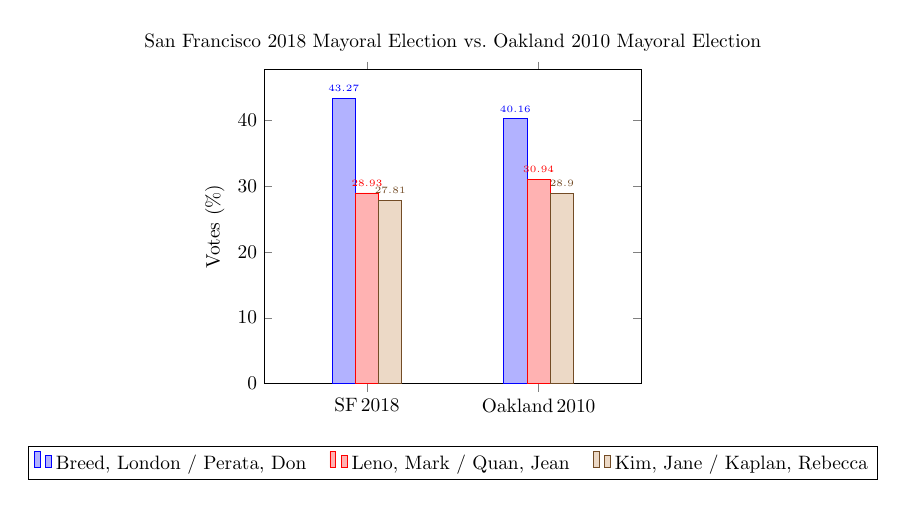
\begin{tikzpicture}[scale=0.7, transform shape]
    \begin{axis}[
      title={San Francisco 2018 Mayoral Election vs.\ Oakland 2010 Mayoral Election},
      ybar,
      bar width=12pt,
      ylabel={Votes (\%)},
      symbolic x coords={SF\,2018,Oakland\,2010},
      xtick=data,
      enlarge x limits=0.6,
      ymin=0,
      enlarge y limits={upper,value=0.1},
      nodes near coords,
      every node near coord/.append style={font=\tiny},
      legend style={
        at={(0.5,-0.20)},
        anchor=north,
        legend columns=3,
        /tikz/every even column/.append style={column sep=1em}
      },
    ] 

      \addplot+[bar shift=-12pt]
        coordinates {(SF\,2018,43.27) (Oakland\,2010,40.16)};
      \addplot+[bar shift=0pt]
        coordinates {(SF\,2018,28.93) (Oakland\,2010,30.94)};
      \addplot+[bar shift=12pt]
        coordinates {(SF\,2018,27.81) (Oakland\,2010,28.90)};

      \legend{
        {Breed, London / Perata, Don},
        {Leno, Mark / Quan, Jean},
        {Kim, Jane / Kaplan, Rebecca}
      }

    \end{axis}
  \end{tikzpicture}
  \label{fig:1}
\end{figure}

Figure \ref{fig:1} compares the vote results for three finalists in the 2018 San Francisco and 2010 Oakland mayoral election. Because the voting preference for the Oakland race in this particular round was comparable to the voting preference in the San Francisco election at the same stage, with Perata led with 40.16\%, versus Breed with 43.27\%; Quan was in second place Quan with 30.94\%, versus Leno with 28.93\%; and Kaplan was in third place with 28.9\%, versus Kim with 27.81\%. 

By Pass 9, Kaplan had in fact received more transferred votes than either Quan or Perata, gaining a 7.32\% increase from the first round, versus 6.47\% increase for Quan and 6.43\% increase for Perata. However, her initial disadvantage still put her on the elimination spot, which turned out to be crucial for Quan’s victory. Of all of Kaplan’s votes, 22.6\% were exhausted, a substantial 19.6\% transferred to Perata, but a decisive 57.7\% went to Quan, pushing her just over the 50\% threshold. 

\section{Conclusion}

Revisiting the three factors – polarization, negative and strategic campaigns, and the spoiler effect, case studies of the 2022 Alaska state Senate and U.S. Senate elections reveal that candidates who appeal to the broader population and less polarized ideas benefit in the RCV elimination rounds; case studies of the 2018 San Francisco and 2010 Oakland mayoral elections reveal that while RCV does not eliminate the presence of strategic voting and utilization of negative ads in the process, it does promotes strategic alliances between candidates, which can be advantageous in the unique RCV elimination process; case studies of 2022 Alaska gubernatorial, state House elections, and U.S. Representative prove that RCV can successfully mitigate the spoiler effect, although the center-squeeze effect potentially prevented third-place moderate candidate Nick Begich from winning the office in the special election for U.S. Representative. 

In 2022, Nevada voters passed a ballot measure to implement a “top-five primary” with open primaries regardless of voter affiliations and a RCV general election to determine the final Representative. The system will take place in the 2024 election season (\cite{clyde2022}, 2022). As RCV implementation expands through years, more observations and conclusions can be made. For example, while this paper can not definitely validate that RCV caused the bipartisan coalition in the Alaska Senate after the 2022 elections, it confirms a correlation between RCV and the incentives for candidates to appeal to bipartisan ideals (\cite{rosen2022}, 2022). As future elections proceed, researchers will have more opportunities to explore how candidate and voter behaviors evolve under RCV, leading to more definitive conclusions. 

In conclusion, this paper posits that RCV can provide tangible meaningful electoral reforms in combating polarization and the spoiler effect. While it can not definitively claim that RCV reduces negative and strategic voting, it does suggest that RCV can visibly moderate candidate behaviors, contributing to a more constructive electoral process.





\printbibliography

\end{document}